\documentclass{beamer}

\usepackage{beamerthemesplit} % Activate for custom appearance


% customize
\usepackage[backend=bibtex]{biblatex}
\bibliography{fpg.bib}
\addbibresource{fpg.bib}
\usepackage{adjustbox}
\usepackage{algorithm}
\usepackage{algorithmic}
\usepackage{tikz}
\usetikzlibrary{decorations.pathmorphing,decorations.markings,trees,positioning,arrows}
\usepackage{multirow} 
\usepackage[french]{babel}
\usepackage{graphicx, float}
\usepackage{geometry}  
\usepackage[toc]{glossaries}
\makeglossaries
\newacronym{fpm}{FPM}{Frequent Pattern Mining}
\newacronym{fp}{FP}{Frequent Pattern}
\newacronym{fpga}{FPGA}{Frequent Pattern Growth Algorithm}
% end customize


\title{Frequent Pattern (FP) Growth Algorithm}
\author{Groupe 1}
\institute[VFU] % (optional)
{
  %\inst{1}%
  UYI\\
  FS\\
  INFO M1\\
  INF4117: Fouille de données
}
\date{\today}

\begin{document}

\frame{\titlepage}

% frame de presentation des membres de l'equipe
\section[Présenté Par:]{}
\frame{
\begin{table}[htp]
\caption{Membres Groupe I}
\begin{center}
\begin{tabular}{|c|c|c|}
\hline
\textbf{Nom} & \textbf{Prénom} & \textbf{Matricule}\\
\hline
BINELI OLA & Mathilda Maguy & 17T2215\\
\hline 
DJIEMBOU TIENTCHEU &Victor Nico & 17T2051\\
\hline
KENFACK TEMGOUA &Vanessa & 17J2871\\
\hline
 \multicolumn{3}{|l|}{\centerline{\textbf{Coordonateur :}}}\\
\hline
\multicolumn{3}{|l|}{\centerline{\textbf{Dr TSOPZE NORBERT}}}\\
\hline
\end{tabular}
\end{center}
\label{Membres Groupe I}
\end{table}%
}

% frame de création de sommaire
%\section[Sommaire]{}
%\frame{\tableofcontents}


% introduction frame
\section{Introduction}
\frame{
\frametitle{Introduction}
\par L'extraction de connaissance dans les bases de données, également appelé \textbf{data mining}, désigne le processus permettant d'extraire des informations et des connaissances utiles qui sont enfouies dans les bases de données, les entrepôts de données (data warehouse) ou autres sources de données.\cite{USDB}
}
\frame{
\par Depuis sa création, le Data Analytique joue un rôle important dans le processus de prise de décision, du coup plusieurs algorithmes \acrfull{fpm} ont été développés pour améliorer les performances d'extraction.\cite{USDB}
\par Durant cette présentation, nous nous intéresserons à l'algorithme de croissance de modèles fréquents dans l'extraction de connaissances.\cite{USDB}
\par Le but de cette étude est de présenter tout d'abord ce que s'est que \textbf{l'Algorithme de croissance de modèles fréquents} (\textit{\acrfull{fp} Growth Algorithm}, en anglais), quels sont les atouts? et quelles sont ses limites?\cite{USDB}
}

% définitio frame
\section{Définitions}
\frame{
\frametitle{Définition}
\textbf{Items:} Est tout objet, article, attribut, littéral appartenant à un ensemble fini d'éléments distincts $I = \{x_1, x_2, x_3, \dots, x_n\}$. En outre, il s'agit d'un ensemble d'attribut de la base de données transactionnelle.
\par \textbf{Itemset:} C'est un ensemble de \textbf{N} items.
\par \textbf{Itemset Frequent:} On dit qu'un itemset est fréquent si et seulement si son support est supérieur à un support minimum définit par l'utilisateur.
\par \textbf{support minimal:} Noté \textbf{Minsup} est le nombre minimum d'occurence d'un itemset pour être considéré comme fréquent.
}
\frame{
\frametitle{Définition}
\par \textbf{Transaction:} Soit $I = \{i_1, i_2, \dots, i_m\}$ un ensemble d’items, D une BD de transactions o\`u chaque transaction T est un sous ensemble de I.
}
%  classification d'algorithme  d'extraction de motifs fréquents
\section[classification d'algorithme  d'extraction de motifs fréquents]{classification d'algorithme  d'extraction de motifs fréquents}
\frame
{
\frametitle{classification d'algorithme  d'extraction de motifs fréquents}

\begin{columns} 

\begin{column}{.3\textwidth}
	\par {\small Les algorithmes d'extraction de motifs fréquents peuvent être classés en deux grandes catégories: \textbf{Algorithmes générer et tester (candidate generate and test) et en croissance de Modèle (pattern growth)}. }
\end{column}

\begin{column}{.7\textwidth}

\begin{figure}[htbp]
\begin{center}
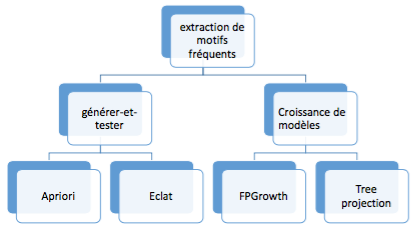
\includegraphics[scale=0.5]{images/class.png}
\caption{classification d'algorithme  d'extraction de motifs fréquents \cite{USDB}}
\label{default}
\end{center}
\end{figure}

\end{column}

\end{columns} 
}

% frame de présentation de problème
\section[Problème]{Problème}
\subsection[Énoncé]{Énoncé}
\frame
{
  \frametitle{Énoncé}
Étant donnée un base de  transactions T, un seuil minimum de support s, le problème est de pouvoir extraire l'ensemble des modèles ou motifs fréquents  tels que le support de chaque itemsets frequents soit supérieur ou égal au minimum de support s définit par l'utilisateur \cite{persoliriscnrs}.
}
\subsection[Exemple d'application réel]{Exemple d'application réel}
\frame
{
  \frametitle{Exemple d'application réel}
Ce problème est communement rencontré dans les domaines tels:
  \begin{itemize}
  \item<1-> \textbf{Dans le domaine de l'éducation: }Extraction des règles d'association dans le data mining des étudiants admis à travers les caractéristiques et les spécialités.  
  \item<1-> \textbf{Dans le domaine médical:} Par exemple, analyse de la base de données des patients.
   \item<1-> \textbf{En foresterie:} Analyse de la probabilité et de l'intensité des feux de forêt avec les données sur les feux de forêt.
   \end{itemize}
 }
 
 \frame
 {
  \frametitle{Exemple d'application réel}
  \begin{itemize}
  \item<1-> \textbf{la fonction de saisie semi-automatique:} par Google
   \item<1-> \textbf{Système de recommandation:} est utilisé par de nombreuses entreprises comme Amazon
   \item<1-> \textbf{Analyse du panier de la ménagère}
   \item<1-> \textbf{Détection des potentiels futurs clients}
   \item<1-> \textbf{Détection de fraude}
  \end{itemize}
}


% frame de solution proposée
\section[Solution proposée]{Solution proposée}
\subsection[Principe]{Principe}
\frame
{
  \frametitle{Principe}
Le principe d'application de l'algorithme \acrfull{fp}  Growth est le suivant: 
  \begin{itemize}
  \item<1-> On effectue un premier parcours de la base de transactions T, pour déterminer les items fréquents en fonction du support minimum fourni. Ces items seront triés par la suite par ordre décroissant de support dans une liste L. Les items ainsi triés seront traités dans cet ordre.\cite{USDB}
  \end{itemize}
  }
\frame
{
  \frametitle{Principe}
  \begin{itemize}
  \item<1-> Un second parcours de T est alors effectué. Chaque transaction est alors trié selon l'ordre des items dans L. Le noeud racine de l'arbre \{null\} est d'abord crée. Durant ce même parcours, une branche sera crée pour chaque transaction, mais les transactions ayant un même préfixe partagerons le même début d'une branche de l'arbre, ainsi deux transactions identiques seront représentées par une et même branche.\cite{USDB} 
  \end{itemize}
}
\subsection[Algorithme]{Algorithme}
\begin{frame}
  \frametitle{Algorithme FP Growth}

\begin{algorithm}[H]
\caption{Frequent Pattern (FP) Growth Algorithm}
\begin{algorithmic}[1]
% header
\REQUIRE un support seuil s et la base  de transactions T.
\ENSURE  liste des itemsets fréquents.

% base treatment
\STATE L $\gets$ liste de items de T dont les support sont $\geq$ s classée suivant s décroissant
\STATE trier T dans l'ordre décroissant de support dans L.
\STATE construire le FP-tree des données transactionnelles de T
\STATE de FP-tree, ressortir le FP-conditional tree pour chaque item (itemset)
\STATE determiner les modèles fréquents.

\end{algorithmic}
\end{algorithm}
\end{frame}

\subsection[Limites]{Limites}
\frame
{
  \frametitle{Limites}
   \begin{itemize}
  \item<1-> L'algorithme de \acrfull{fp} Growth résout le problème de la nécessité de nombreuses analyses de la base de données, vue qu'il ne fait que deux balayages de la base de transactions. \cite{towardsdatascience}
  \item<1-> Neanmoins, cela ne garantit pas, dans le cas où la base de transactions est trop volumineuse, que toute la structure du FP-tree tiendra en mémoire central \cite{softwaretestinghelp}. De plus la construction du FP-tree peut s'avérer longue et pourrait consommer beaucoup de ressources système.\cite{mygreatlearning}
  \end{itemize}

}

% frame de présentation d'un exemple d'application réel
% exemple définition
\section[Exemple]{Exemple}
\frame
{
  \frametitle{Exemple}
  {\small Soit donnée la base de transaction T ci-dessous et s = 2 le minimum de support. Trouvons tout les motifs fréquents en utilisant l'algorithme de croissance de modèles frequents.}

\begin{columns} 
% Column 1
   {\small  \begin{column}{.5\textwidth}
        Dans cette base, les différents caractères sont des substituants d'articles dans un carrefour.\cite{towardsdatascience}
     	  \begin{itemize}
 		 \item<1-> A: bièrre
		 \item<1-> B: vin
		 \item<1-> C: chips
		 \item<1-> D: oeuf
		 \item<1-> E: fleur
  	\end{itemize}
    \end{column}
% Column 2    
    \begin{column}{.5\textwidth}
  			\begin{table}[htp]
			\caption{Base de transactions}
			\begin{center}
				\begin{tabular}{|c|c|}
				\hline
				\textbf{T} & \textbf{Items} \\
				\hline
				1 & A,B \\
				\hline
				2 & B, C, D \\
				\hline
				3 & A, C, D, E \\
				\hline
				4 & A, D, E \\
				\hline
				5 & A, B, C \\
				\hline
				\end{tabular}
			\end{center}
			\label{Base de transactions}
			\end{table}%
    \end{column}%
   }
\end{columns}  

  }
  
  % step 1 et 2 implémentation
\frame
{
  \frametitle{Exemple: étape 1 et 2}
 
 \begin{columns} 
% step 1  implémentation
    \begin{column}{.5\textwidth}
  			\begin{table}[htp]
			\caption{Liste des items frequents de T }
			\begin{center}
				\begin{tabular}{|c|c|}
				\hline
				\textbf{L} & \textbf{Support} \\
				\hline
				A & 4\\
				\hline
				B & 3 \\
				\hline
				C & 3 \\
				\hline
				D & 3 \\
				\hline
				E & 2 \\
				\hline
				\end{tabular}
			\end{center}
			\label{Liste des items frequents de T }
			\end{table}%
    \end{column}
% Column 2    
    \begin{column}{.5\textwidth}
  			\begin{table}[htp]
			\caption{Base de transactions  suivant L}
			\begin{center}
				\begin{tabular}{|c|c|}
				\hline
				\textbf{T} & \textbf{Ordered Frequent Items} \\
				\hline
				1 & A,B \\
				\hline
				2 & B, C, D \\
				\hline
				3 & A, C, D, E\\
				\hline
				4 & A, D, E \\
				\hline
				5 & A, B, C \\
				\hline
				\end{tabular}
			\end{center}
			\label{Base de transactions suivant L}
			\end{table}%
    \end{column}%
    
\end{columns}
}

  % step 3 
  % substep i)
\frame
{
  \frametitle{Exemple: étape 3 i) }

 \begin{columns} 
% substep i)
    \begin{column}{.5\textwidth}
    Constuire le FP-tree   et ajouter T1.\\
  			\begin{table}[htp]
			\caption{Base de transactions  suivant L}
			\begin{center}
				\begin{tabular}{|c|c|}
				\hline
				\textbf{T} & \textbf{Ordered Frequent Items} \\
				\hline
				1 & A,B \\
				\hline
				\end{tabular}
			\end{center}
			\label{Base de transactions suivant L}
			\end{table}%    

    \end{column}
% Column 2    
    \begin{column}{.5\textwidth}
        \begin{tikzpicture}[sibling distance=6em,level distance=4em,every node/.style={shape=rectangle,draw,align=center}]
 
\node [circle, fill=white, minimum size = 4pt, inner sep = 0] {root}
    child {node [circle, fill=white, minimum size = 4pt, inner sep = 0] {$A:1$}
    	child {node [circle, fill=white, minimum size = 4pt, inner sep = 0] {$B:1$}}
    };
 
\end{tikzpicture}
    \end{column}%
    
\end{columns}
}  

  % step 3 
  % substep ii)
\frame
{
  \frametitle{Exemple : étape 3 ii) }

 \begin{columns} 
% step 1  implémentation
    \begin{column}{.5\textwidth}
    Ajouter T2 dans  le FP-tree transaction de la base T.\\
  			\begin{table}[htp]
			\caption{Base de transactions  suivant L}
			\begin{center}
				\begin{tabular}{|c|c|}
				\hline
				\textbf{T} & \textbf{Ordered Frequent Items} \\
				\hline
				1 & A,B \\
				\hline
				2 & B,C,D \\
				\hline
				\end{tabular}
			\end{center}
			\label{Base de transactions suivant L}
			\end{table}%    

    \end{column}
% Column 2    
    \begin{column}{.5\textwidth}
        \begin{tikzpicture}[sibling distance=6em,level distance=4em,every node/.style={shape=rectangle,draw,align=center,decorate},every edge/.style={shape=rectangle,draw,align=center,decorate,postaction={decorate,decoration={markings,mark=at position 1 with {\arrow[draw=black]{>}}}}}]
 
\node [circle, fill=white, minimum size = 4pt, inner sep = 0] (root){root}
    child {node [circle, fill=white, minimum size = 4pt, inner sep = 0] (A1){$A:1$}
    	child {node [circle, fill=white, minimum size = 4pt, inner sep = 0] (B1){$B:1$}}
    }
    child {node [circle, fill=white, minimum size = 4pt, inner sep = 0] (B2){$B:1$}
    	child {node [circle, fill=white, minimum size = 4pt, inner sep = 0] (C1){$C:1$}
		child {node [circle, fill=white, minimum size = 4pt, inner sep = 0] (D1){$D:1$}}
	}
    };
    \path[draw=black,thick,dashed] (B1) edge[bend left] (B2);
    \path[draw=black] (root) edge(B2);
     \path[draw=black] (root) edge(A1);
      \path[draw=black] (A1) edge(B1);
       \path[draw=black] (B2) edge(C1);
        \path[draw=black] (C1) edge(D1);
 
\end{tikzpicture}
    \end{column}%
    
\end{columns}
}  

  % step 3 
  % substep iii)
\frame
{
  \frametitle{Exemple : étape 3 iii) }

 \begin{columns} 
% step 1  implémentation
    \begin{column}{.5\textwidth}
    Ajouter T3 dans  le FP-tree transaction de la base T.\\
  			\begin{table}[htp]
			\caption{Base de transactions  suivant L}
			\begin{center}
				\begin{tabular}{|c|c|}
				\hline
				\textbf{T} & \textbf{Ordered Frequent Items} \\
				\hline
				1 & A,B \\
				\hline
				2 & B,C,D \\
				\hline
				3 & A,C,D, E \\
				\hline
				\end{tabular}
			\end{center}
			\label{Base de transactions suivant L}
			\end{table}%    

    \end{column}
% Column 2    
    \begin{column}{.5\textwidth}
        \begin{tikzpicture}[sibling distance=6em,level distance=3em,every node/.style={shape=rectangle,draw,align=center,decorate},every edge/.style={shape=rectangle,draw,align=center,decorate,postaction={decorate,decoration={markings,mark=at position 1 with {\arrow[draw=black]{>}}}}},
level 1/.style={sibling distance=28mm},
level 2/.style={sibling distance=14mm},
level 3/.style={sibling distance= 6mm},
level 4/.style={sibling distance= 4mm},]
 
\node [circle, fill=white, minimum size = 4pt, inner sep = 0] (root){root}
    child {node [circle, fill=white, minimum size = 4pt, inner sep = 0] (A1){$A:2$}
    	child {node [circle, fill=white, minimum size = 4pt, inner sep = 0] (B1){$B:1$}}
	child {node [circle, fill=white, minimum size = 4pt, inner sep = 0] (C2){$C:1$}
		child {node [circle, fill=white, minimum size = 4pt, inner sep = 0] (D2){$D:1$}
			child {node [circle, fill=white, minimum size = 4pt, inner sep = 0] (E1){$E:1$}}
		}
	}
    }
    child {node [circle, fill=white, minimum size = 4pt, inner sep = 0] (B2){$B:1$}
    	child {node [circle, fill=white, minimum size = 4pt, inner sep = 0] (C1){$C:1$}
		child {node [circle, fill=white, minimum size = 4pt, inner sep = 0] (D1){$D:1$}}
	}
    };
    \path[draw=black,thick,dashed] (B1) edge(B2);
    \path[draw=black,thick,dashed] (C2) edge(C1);
    \path[draw=black,thick,dashed] (D2) edge(D1);
    \path[draw=black] (root) edge(B2);
     \path[draw=black] (root) edge(A1);
      \path[draw=black] (A1) edge(B1);
      \path[draw=black] (A1) edge(C2);
       \path[draw=black] (B2) edge(C1);
        \path[draw=black] (C1) edge(D1);
        \path[draw=black] (C2) edge(D2);
      \path[draw=black] (D2) edge(E1);
 
\end{tikzpicture}
    \end{column}%
    
\end{columns}
}
  % step 3 
  % substep iv)
\frame
{
  \frametitle{Exemple : étape 3 iv) }

 \begin{columns} 
% step 1  implémentation
    \begin{column}{.5\textwidth}
    Ajouter T4 dans  le FP-tree transaction de la base T.
  			\begin{table}[htp]
			\caption{Base de transactions  suivant L}
			\begin{center}
				\begin{tabular}{|c|c|}
				\hline
				\textbf{T} & \textbf{Ordered Frequent Items} \\
				\hline
				1 & A,B \\
				\hline
				2 & B,C,D \\
				\hline
				3 & A,C,D, E \\
				\hline
				4 & A,D, E \\
				\hline
				\end{tabular}
			\end{center}
			\label{Base de transactions suivant L}
			\end{table}%    

    \end{column}
% Column 2    
    \begin{column}{.5\textwidth}
        \begin{tikzpicture}[sibling distance=4em,level distance=3em,
        every node/.style={shape=rectangle,draw,align=center,decorate},
        node/.style={shape=rectangle,draw,align=center,decorate},
        every edge/.style={shape=rectangle,draw,align=center,decorate,postaction={decorate,decoration={markings,mark=at position 1 with {\arrow[draw=black]{>}}}}},
level 1/.style={sibling distance=28mm},
level 2/.style={sibling distance=14mm},
level 3/.style={sibling distance= 6mm},
level 4/.style={sibling distance= 4mm},
        ]
 
\node [circle, fill=white, minimum size = 4pt, inner sep = 0] (root){root}
    child {node [circle, fill=white, minimum size = 4pt, inner sep = 0] (A1){$A:3$}
    	child {node [circle, fill=white, minimum size = 4pt, inner sep = 0] (B1){$B:1$}}
	child {node [circle, fill=white, minimum size = 4pt, inner sep = 0] (C2){$C:1$}
		child {node [circle, fill=white, minimum size = 4pt, inner sep = 0] (D2){$D:1$}
			child {node [circle, fill=white, minimum size = 4pt, inner sep = 0] (E1){$E:1$}}
		}
	}
	child {node [circle, fill=white, minimum size = 4pt, inner sep = 0] (D3){$D:1$}
		child {node [circle, fill=white, minimum size = 4pt, inner sep = 0] (E2){$E:1$}}
	}
    }
    %child {node [circle, fill=white, minimum size = 4pt, inner sep = 0] {}}
    %child {node [circle, fill=white, minimum size = 4pt, inner sep = 0] (D3){$D:1$}}
    child {node [circle, fill=white, minimum size = 4pt, inner sep = 0, sibling distance = 10em] (B2){$B:1$}
    	child {node [circle, fill=white, minimum size = 4pt, inner sep = 0] (C1){$C:1$}
		child {node [circle, fill=white, minimum size = 4pt, inner sep = 0] (D1){$D:1$}}
	}
    };
    \path[draw=black,thick,dashed] (B1) edge(B2);
    \path[draw=black,thick,dashed] (C2) edge[bend left](C1);
    \path[draw=black,thick,dashed] (D2) edge(D3);
    \path[draw=black,thick,dashed] (D3) edge(D1);
    \path[draw=black,thick,dashed] (E1) edge(E2);
    
    \path[draw=black] (root) edge(B2);
     \path[draw=black] (root) edge(A1);
     
      \path[draw=black] (A1) edge(B1);
      \path[draw=black] (A1) edge(C2);
      \path[draw=black] (A1) edge(D3);
      
       \path[draw=black] (B2) edge(C1);
       
        \path[draw=black] (C1) edge(D1);
 
\end{tikzpicture}
    \end{column}%
    
\end{columns}
}
  % step 3 
  % substep v)
\frame
{
  \frametitle{Exemple  : étape 3 v) }

 \begin{columns} 
% step 1  implémentation
    \begin{column}{.5\textwidth}
    Ajouter T5 dans le FP-tree transaction de la base T.
  			\begin{table}[htp]
			\caption{Base de transactions  suivant L}
			\begin{center}
				\begin{tabular}{|c|c|}
				\hline
				\textbf{T} & \textbf{Ordered Frequent Items} \\
				\hline
				1 & A,B \\
				\hline
				2 & B,C,D \\
				\hline
				3 & A,C,D, E \\
				\hline
				4 & A,D, E \\
				\hline
				5 & A,B,C \\
				\hline
				\end{tabular}
			\end{center}
			\label{Base de transactions suivant L}
			\end{table}%    

    \end{column}
% Column 2    
    \begin{column}{.5\textwidth}
        \begin{tikzpicture}[sibling distance=4em,level distance=3em,
        every node/.style={shape=rectangle,draw,align=center,decorate},
        node/.style={shape=rectangle,draw,align=center,decorate},
        every edge/.style={shape=rectangle,draw,align=center,decorate,postaction={decorate,decoration={markings,mark=at position 1 with {\arrow[draw=black]{>}}}}},
level 1/.style={sibling distance=28mm},
level 2/.style={sibling distance=14mm},
level 3/.style={sibling distance= 6mm},
level 4/.style={sibling distance= 4mm},
        ]
 
\node [circle, fill=white, minimum size = 4pt, inner sep = 0] (root){root}
    child {node [circle, fill=white, minimum size = 4pt, inner sep = 0] (A1){$A:4$}
    	child {node [circle, fill=white, minimum size = 4pt, inner sep = 0] (B1){$B:2$}
		child {node [circle, fill=white, minimum size = 4pt, inner sep = 0] (C3){$C:1$}}
	}
	child {node [circle, fill=white, minimum size = 4pt, inner sep = 0] (C2){$C:1$}
		child {node [circle, fill=white, minimum size = 4pt, inner sep = 0] (D2){$D:1$}
			child {node [circle, fill=white, minimum size = 4pt, inner sep = 0] (E1){$E:1$}}
		}
	}
	child {node [circle, fill=white, minimum size = 4pt, inner sep = 0] (D3){$D:1$}
		child {node [circle, fill=white, minimum size = 4pt, inner sep = 0] (E2){$E:1$}}
	}
    }
    child {node [circle, fill=white, minimum size = 4pt, inner sep = 0, sibling distance = 10em] (B2){$B:1$}
    	child {node [circle, fill=white, minimum size = 4pt, inner sep = 0] (C1){$C:1$}
		child {node [circle, fill=white, minimum size = 4pt, inner sep = 0] (D1){$D:1$}}
	}
    };
    \path[draw=black,thick,dashed] (B1) edge(B2);
    \path[draw=black,thick,dashed] (C2) edge[bend left](C1);
    \path[draw=black,thick,dashed] (D2) edge(D3);
    \path[draw=black,thick,dashed] (D3) edge(D1);
    \path[draw=black,thick,dashed] (E1) edge(E2);
    \path[draw=black,thick,dashed] (C3) edge(C2);
    
    \path[draw=black] (root) edge(B2);
     \path[draw=black] (root) edge(A1);
     
      \path[draw=black] (A1) edge(B1);
      \path[draw=black] (A1) edge(C2);
      \path[draw=black] (A1) edge(D3);
      
      \path[draw=black] (B1) edge(C3);
      
       \path[draw=black] (B2) edge(C1);
       
        \path[draw=black] (C1) edge(D1);
 
\end{tikzpicture}
    \end{column}%
    
\end{columns}
}

  % step 3 
  % substep v)
\frame
{
  \frametitle{Exemple : étape 4 }
Trouver les itemsets fréquents.
    
  			\begin{table}[htp]
			\caption{Extraction de motifs frequents}
			\begin{center}
				\begin{adjustbox}{width=\columnwidth,center}
				\begin{tabular}{|c|c|c|c|}
				\hline
				\textbf{Item} & \textbf{Conditional Pattern base} & \textbf{Conditional FP-tree} & \textbf{Frequent Pattern Generated} \\
				\hline
				E & $\{\{A,C,D:1\},\{A,D:1\}\}$ & 
				$\langle A:2 \rangle,\langle D:2\rangle$ & 
				$\{E,A:2\},\{E,D:2\},\{E,A,D:2\}$  \\
				\hline
				D & $\{\{A,C:1\},\{A:1\},\{B,C:1\}\}$ & 
				$\langle A:2\rangle$ & 
				$\{D,A:2\}$  \\
				\hline
				C & $\{\{A,B:1\},\{A:1\},\{B:1\}\}$ & 
				$\langle A:2\rangle$ & 
				$\{C,A:2\}$  \\
				\hline
				B & $\{\{A:2\}\}$ & 
				$\langle A:2\rangle$ & 
				$\{B,A:2\}$ \\
				\hline
				\end{tabular}
				\end{adjustbox}
			\end{center}
			\label{Base de transactions suivant L}
			\end{table}%    
}

% remerciement.
\section[Résumé]{Résumé}
\frame
{
\frametitle{Résumé}
\begin{figure}[htbp]
\begin{center}

\includegraphics[scale=0.7]{images/sum.jpeg}
%\caption{Merci}
\label{summary}
\end{center}
\end{figure}
}

% references
{\small \begin{frame}[noframenumbering,plain,allowframebreaks]{Référence}
\printbibliography
\end{frame}}
% remerciement.
\section[Remerciement]{Remerciement}
\frame
{
\frametitle{Fin}
\begin{figure}[htbp]
\begin{center}

\includegraphics[scale=0.7]{images/thanks.jpeg}
%\caption{Merci}
\label{Remerciement}
\end{center}
\end{figure}
}


\end{document}
